%!TEX TS-program = xelatex
\documentclass[notes,12pt, aspectratio=169]{beamer}

\usepackage{amsmath,amsfonts,amssymb,amsthm,mathtools}  % пакеты для математики

\usepackage[english, russian]{babel} % выбор языка для документа
\usepackage[utf8]{inputenc} % задание utf8 кодировки исходного tex файла
\usepackage[X2,T2A]{fontenc}        % кодировка

\usepackage{fontspec}         % пакет для подгрузки шрифтов
\setmainfont{Helvetica}  % задаёт основной шрифт документа

% why do we need \newfontfamily:
% http://tex.stackexchange.com/questions/91507/
\newfontfamily{\cyrillicfonttt}{Helvetica}
\newfontfamily{\cyrillicfont}{Helvetica}
\newfontfamily{\cyrillicfontsf}{Helvetica}

\usepackage{unicode-math}     % пакет для установки математического шрифта
% \setmathfont{Neo Euler} % шрифт для математики

\usepackage{polyglossia}      % Пакет, который позволяет подгружать русские буквы
\setdefaultlanguage{russian}  % Основной язык документа
\setotherlanguage{english}    % Второстепенный язык документа

% Шрифт для кода
\setmonofont[Scale=0.85]{Monaco}
\usepackage{verbments}

\usepackage{pgfpages}
% These slides also contain speaker notes. You can print just the slides,
% just the notes, or both, depending on the setting below. Comment out the want
% you want.
%\setbeameroption{hide notes} % Only slide
%\setbeameroption{show only notes} % Only notes
%\setbeameroption{show notes on second screen=right} % Both

\usepackage{array}

\usepackage{tikz}
\usepackage{verbatim}
\setbeamertemplate{note page}{\pagecolor{yellow!5}\insertnote}
\usetikzlibrary{positioning}
\usetikzlibrary{snakes}
\usetikzlibrary{calc}
\usetikzlibrary{arrows}
\usetikzlibrary{decorations.markings}
\usetikzlibrary{shapes.misc}
\usetikzlibrary{matrix,shapes,arrows,fit,tikzmark}

\usepackage{hyperref}
\usepackage{lipsum}
\usepackage{multimedia}
\usepackage{multirow}
\usepackage{dcolumn}
\usepackage{bbm}
\newcolumntype{d}[0]{D{.}{.}{5}}

\usepackage{changepage}
\usepackage{appendixnumberbeamer}
\newcommand{\beginbackup}{
   \newcounter{framenumbervorappendix}
   \setcounter{framenumbervorappendix}{\value{framenumber}}
   \setbeamertemplate{footline}
   {
     \leavevmode%
     \hline
     box{%
       \begin{beamercolorbox}[wd=\paperwidth,ht=2.25ex,dp=1ex,right]{footlinecolor}%
%         \insertframenumber  \hspace*{2ex} 
       \end{beamercolorbox}}%
     \vskip0pt%
   }
 }
\newcommand{\backupend}{
   \addtocounter{framenumbervorappendix}{-\value{framenumber}}
   \addtocounter{framenumber}{\value{framenumbervorappendix}} 
}

% для имитации питоновского синтаксиса 
\newcommand{\pgr}[1]{{\color{green} \textbf{#1}}}


%%%%%%%%%% Работа с картинками %%%%%%%%%
\usepackage{graphicx}                  % Для вставки рисунков
\usepackage{graphics}
\graphicspath{{../images/}}    % можно указать папки с картинками
\usepackage{wrapfig}                   % Обтекание рисунков и таблиц текстом

\usepackage[space]{grffile}
\usepackage{booktabs}

\usepackage{fontawesome5}
\usepackage{bbding}

% These are my colors -- there are many like them, but these ones are mine.
\definecolor{blue}{RGB}{0,114,178}
\definecolor{red}{RGB}{213,94,0}
\definecolor{yellow}{RGB}{240,228,66}
\definecolor{green}{RGB}{0,128, 0}

\hypersetup{
  colorlinks=true,
  linkbordercolor = {white},
  linkcolor = {blue},
  urlcolor= {blue}
}


%% I use a beige off white for my background
\definecolor{MyBackground}{RGB}{255,253,218}

%% Uncomment this if you want to change the background color to something else
%\setbeamercolor{background canvas}{bg=MyBackground}

%% Change the bg color to adjust your transition slide background color!
\newenvironment{transitionframe}{
  \setbeamercolor{background canvas}{bg=yellow}
  \begin{frame}}{
    \end{frame}
}

\setbeamercolor{frametitle}{fg=blue}
\setbeamercolor{title}{fg=black}
\setbeamertemplate{footline}[frame number]
\setbeamertemplate{navigation symbols}{} 
\setbeamertemplate{itemize items}{-}
\setbeamercolor{itemize item}{fg=blue}
\setbeamercolor{itemize subitem}{fg=blue}
\setbeamercolor{enumerate item}{fg=blue}
\setbeamercolor{enumerate subitem}{fg=blue}
\setbeamercolor{button}{bg=MyBackground,fg=blue,}


% If you like road maps, rather than having clutter at the top, have a roadmap show up at the end of each section 
% (and after your introduction)
% Uncomment this is if you want the roadmap!
% \AtBeginSection[]
% {
%    \begin{frame}
%        \frametitle{Roadmap of Talk}
%        \tableofcontents[currentsection]
%    \end{frame}
% }
\setbeamercolor{section in toc}{fg=blue}
\setbeamercolor{subsection in toc}{fg=red}
\setbeamersize{text margin left=1em,text margin right=1em} 

% списки, которые растягиваются на всю величину слайда 
\newenvironment{wideitemize}{\itemize\addtolength{\itemsep}{10pt}}{\enditemize}


\usepackage{xcolor}

% Syntax: \colorboxed[<color model>]{<color specification>}{<math formula>}
\newcommand*{\colorboxed}{}
\def\colorboxed#1#{%
	\colorboxedAux{#1}%
}

\newcommand*{\colorboxedAux}[3]{%
	% #1: optional argument for color model
	% #2: color specification
	% #3: formula
	\begingroup
	\colorlet{cb@saved}{.}%
	\color#1{#2}%
	\boxed{%
		\color{cb@saved}%
		#3%
	}%
	\endgroup
}

\usepackage{pgfplots}
\usepackage{tikz}

\DeclareMathOperator{\logloss}{logloss}

\title[]{\textcolor{blue}{Анализ данных в R}}
\date{\today}

\usepackage{ulem}

\begin{document}

%%% TIKZ STUFF
\tikzset{   
        every picture/.style={remember picture,baseline},
        every node/.style={anchor=base,align=center,outer sep=1.5pt},
        every path/.style={thick},
        }
\newcommand\marktopleft[1]{%
    \tikz[overlay,remember picture] 
        \node (marker-#1-a) at (-.3em,.3em) {};%
}
\newcommand\markbottomright[2]{%
    \tikz[overlay,remember picture] 
        \node (marker-#1-b) at (0em,0em) {};%
}
\tikzstyle{every picture}+=[remember picture] 
\tikzstyle{mybox} =[draw=black, very thick, rectangle, inner sep=10pt, inner ysep=20pt]
\tikzstyle{fancytitle} =[draw=black,fill=red, text=white]
%%%% END TIKZ STUFF

% Title Slide

\begin{frame}
\maketitle
\end{frame}

\begin{frame}{Pipeline анализа данных}
	
	\begin{center}
		Получение и импорт данных \\ 
		\textcolor{red}{$\Downarrow$} \\ 
		Первичный анализ и визуализация \\
		\textcolor{red}{$\Downarrow$} \\ 
		Очистка данных \\
		\textcolor{red}{$\Downarrow$} \\ 
		Трансформация данных \\
		\textcolor{red}{$\Downarrow$} \\ 
		Построение модели
	\end{center}

\end{frame}

\begin{transitionframe}
	\begin{center}
		\Huge Импорт 
	\end{center}
\end{transitionframe}

\begin{frame}{Откуда приходят данные}
	\centering 
\includegraphics[scale = 0.45]{ris.png}
\end{frame}

\begin{frame}{Какими бывают данные}
	\begin{wideitemize}
		\item \textcolor{red}{Cross-sectional} $-$ матрица объекты-признаки за фиксированный период времени
		\item \textcolor{red}{Time series} $-$ данные о каком-то объкте в разные периоды времени
		\item \textcolor{red}{Panel data} $-$ матрица объекты-признаки в разные периоды времени
	\end{wideitemize}
\end{frame}

\begin{frame}{Какими бывают данные}
	\centering 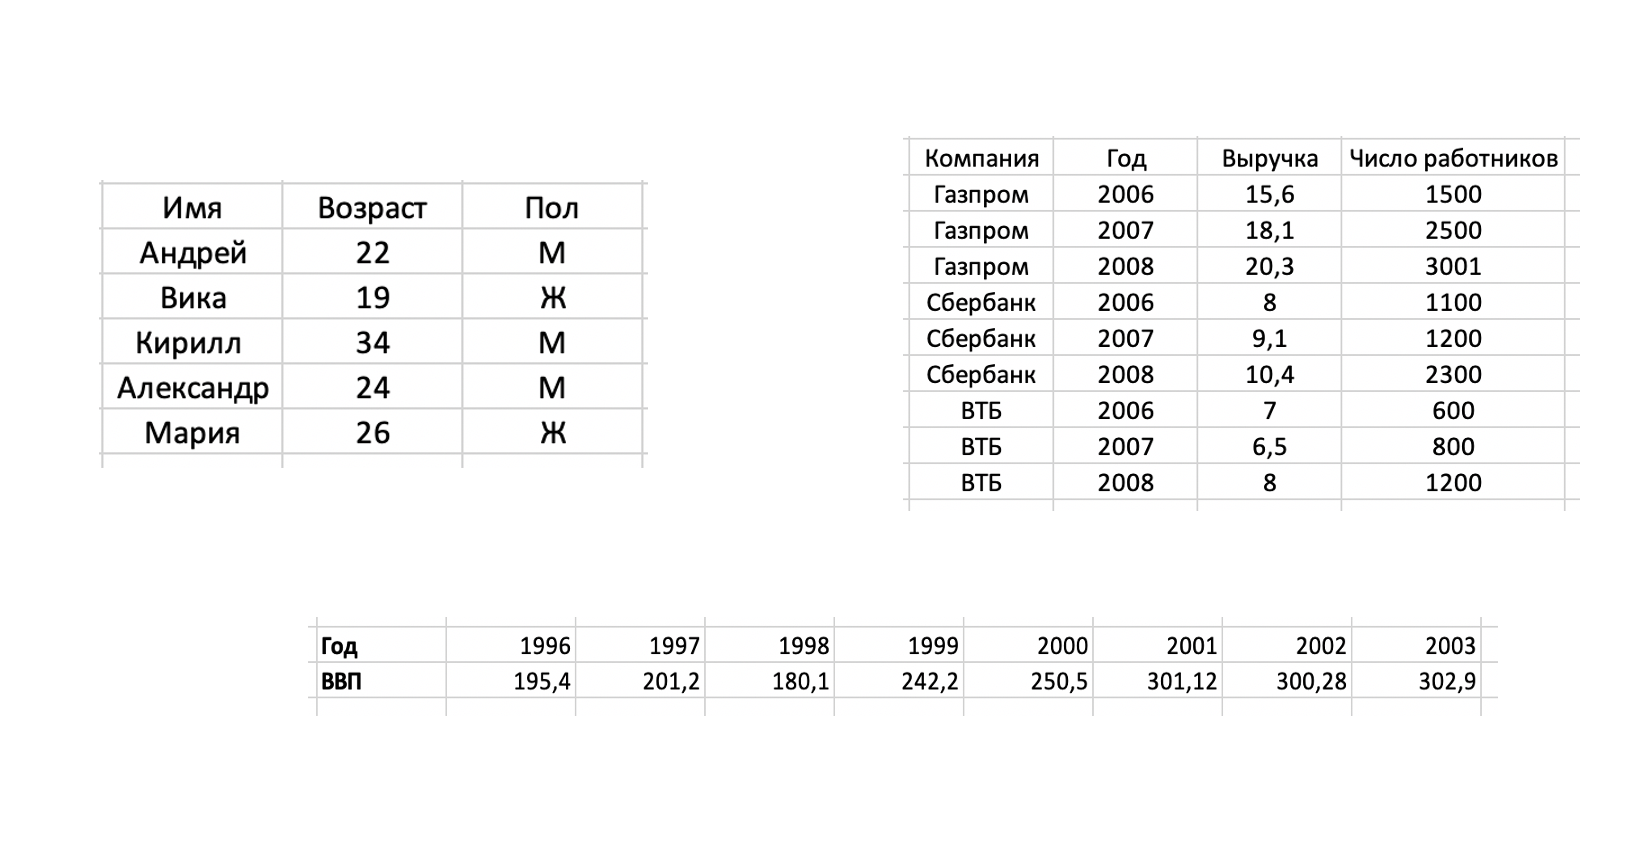
\includegraphics[scale = 0.45]{ris2.png}
\end{frame}

\begin{frame}{Немного про обозначения}
	\centering 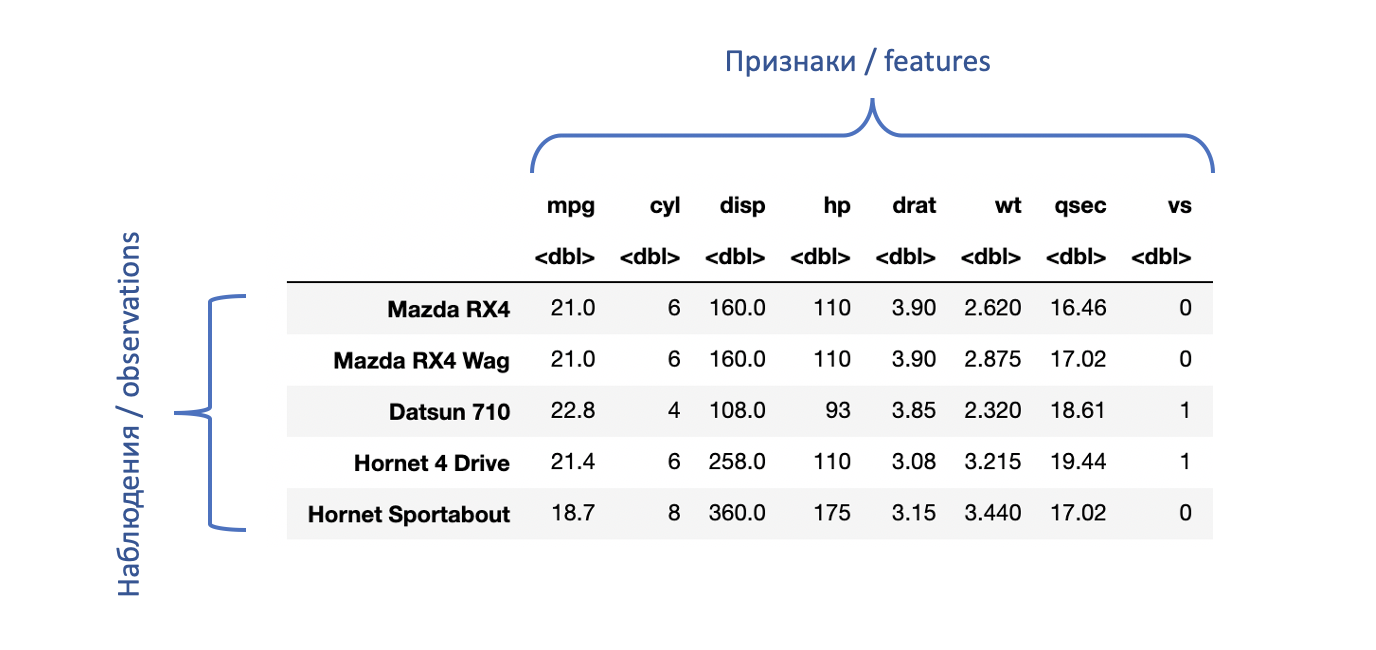
\includegraphics[scale = 0.45]{ris3.png}
	\begin{wideitemize}
		\item Вся таблица $-$ матрица (или так называемый DataFrame)
		\item Один столбец в DataFrame $-$ массив, имеющий данные одного типа 
	\end{wideitemize}
\end{frame}

\begin{frame}{Типы данных}
	\begin{wideitemize}
		\item \textcolor{red}{Числовые (int/dbl)} $-$ целые или вещественные числа
		\item \textcolor{red}{Строковые} $-$ текст
		\item \textcolor{red}{Бинарные} $-$ состоящие из двух категорий (1/0; Да/Нет; TRUE/FALSE)
		\item \textcolor{red}{Категориальные} $-$ состоящие из нескольких категорий (1/2/3; Москва/Лондон/Париж)
		\item \textcolor{red}{DateTime} $-$ специальный формат, связанный со временем и датой
	\end{wideitemize}
\end{frame}

\begin{transitionframe}
	\begin{center}
		\Huge Первичный анализ
	\end{center}
\end{transitionframe}

\begin{frame}{Статистики}
	Хотим посмотреть на закономерности в данных!
	\begin{wideitemize}
		\item \textcolor{red}{Среднее} $-$ простое среднее арифметическое $\bar{x} = \frac{\sum_{i=1}^{n}x_i}{n}$
		\item \textcolor{red}{Дисперсия} $-$ степень разброса значений около среднего $Var = \sum_{i=1}^{n} (x_i - \bar{x})^2$
		\item \textcolor{red}{Среднеквадратическое отклонение} $-$ корень из дисперсии $\sqrt{Var} = \sqrt{\sum_{i=1}^{n} (x_i - \bar{x})^2}$
		\item \textcolor{red}{Квантиль} $-$ значение, которое случайная величина не превышает с фиксированной вероятностью
		\item \textcolor{red}{Медиана} $-$ значение, для которого 50\% значений в выборке находится ниже и 50\% выше. По сути это 50\% квантиль 
		\item \textcolor{red}{Максимум и минимум}
	\end{wideitemize}
\end{frame}

\begin{frame}{Немного о распределениях}
	\begin{wideitemize}
		\item \textcolor{red}{Функция распределения случайной величины $X$} $-$ это вероятность того, что случайная величина $X$ примет значение, меньшее или равное $x$, где $x$ $-$ произвольное действительное число
		\item \textcolor{red}{Плотность распределения случайной величины $X$} $-$ производная от функции распеределения. По сути она показывает какую-то среднюю вероятность, приходящую на бесконечно малый отрезок
	\end{wideitemize}
\end{frame}

\begin{frame}{Немного о распределениях}
	\centering 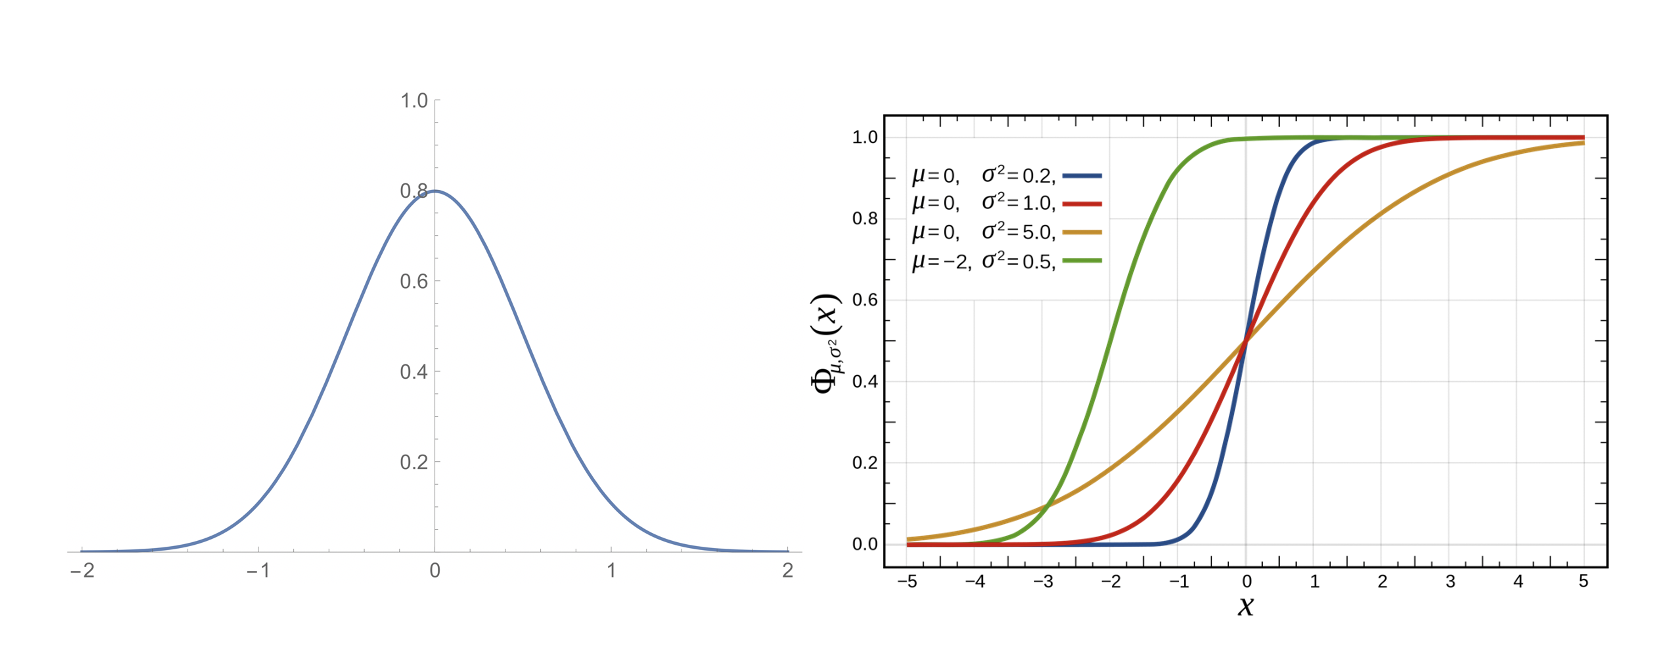
\includegraphics[scale = 0.5]{ris4.png}
\end{frame}

\begin{frame}{Возможности ggplot}
	\centering 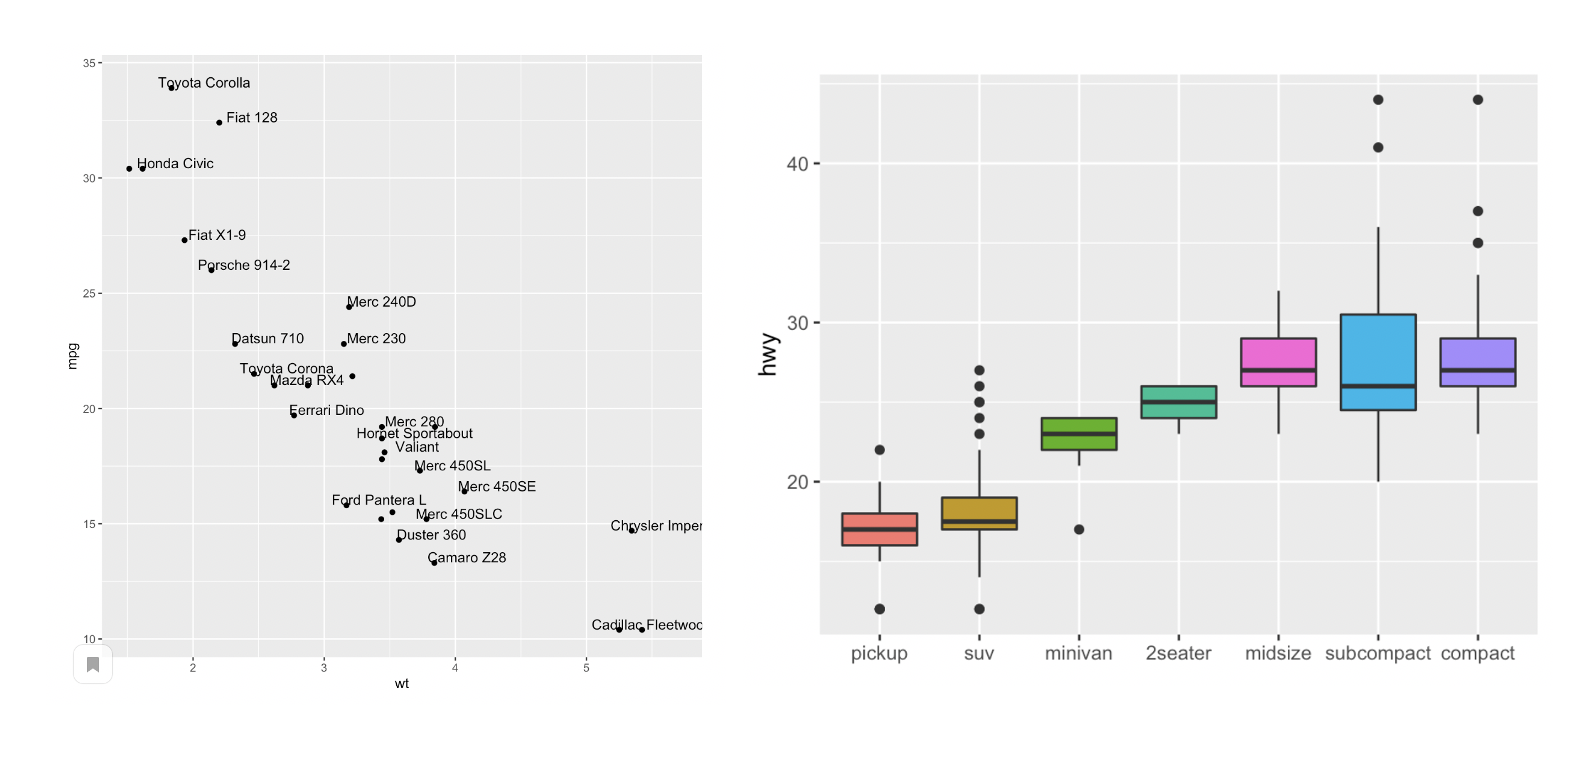
\includegraphics[scale = 0.5]{ris5.png}
\end{frame}

\begin{frame}{Возможности ggplot}
	\centering 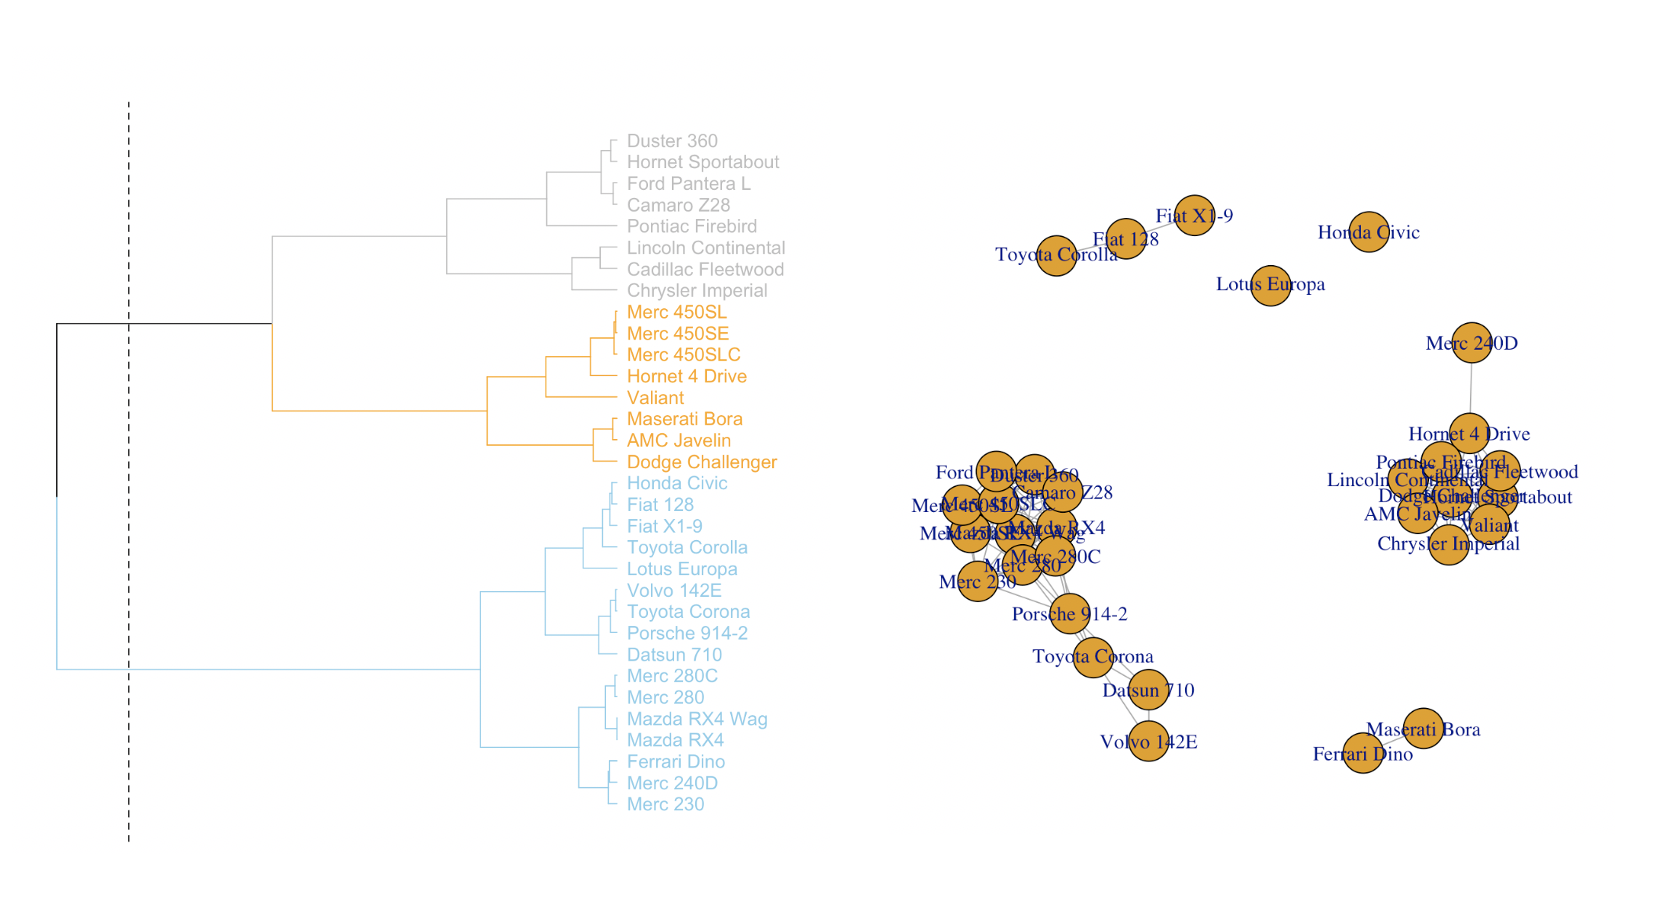
\includegraphics[scale = 0.45]{ris6.png}
\end{frame}

\begin{frame}{Возможности ggplot}
	\centering 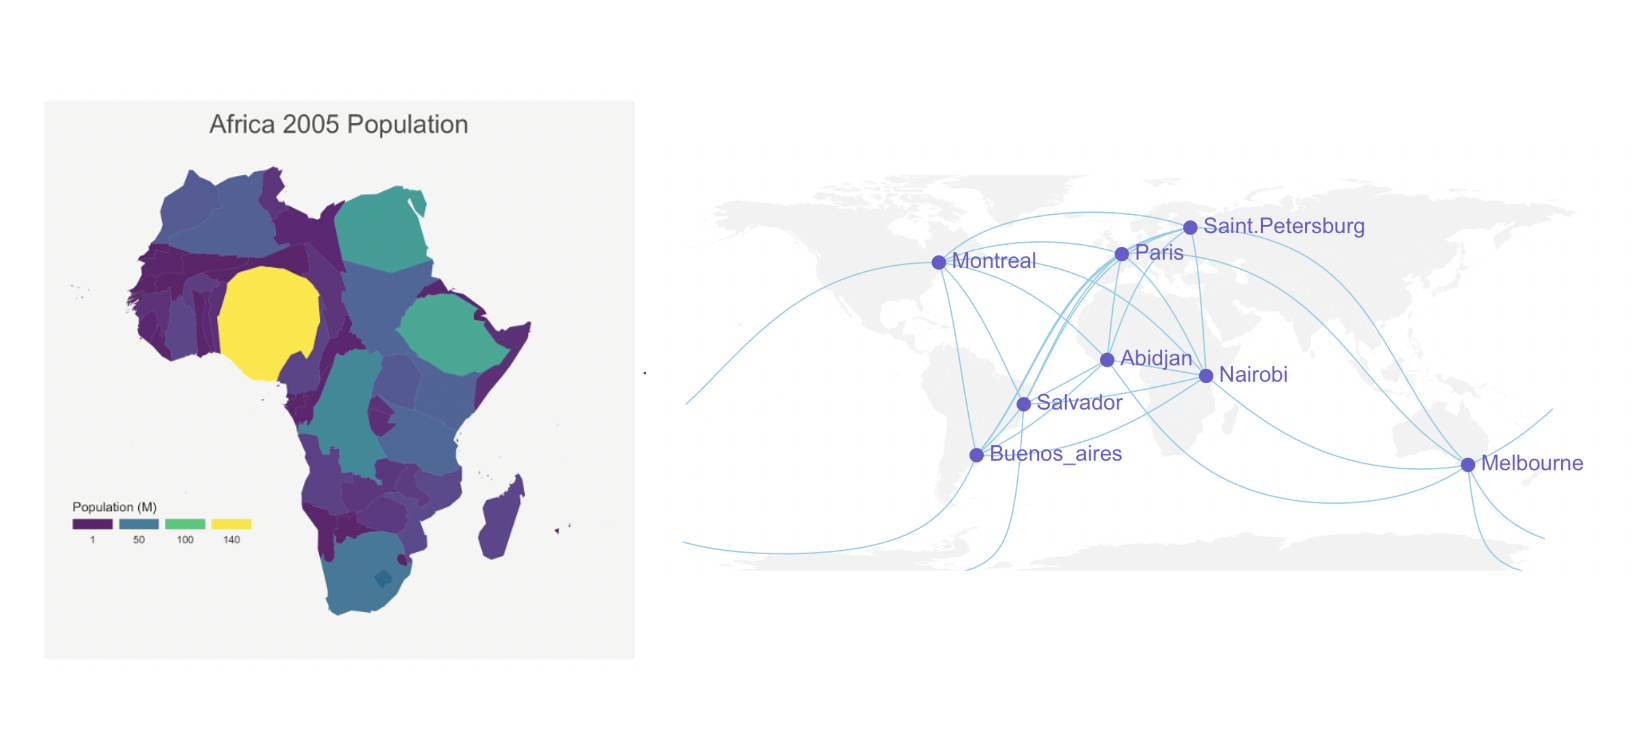
\includegraphics[scale = 0.5]{ris7.png}
\end{frame}

\begin{transitionframe}
	\begin{center}
		\Huge Очистка данных
	\end{center}
\end{transitionframe}

\begin{frame}{Проблемы опросников}
	\centering 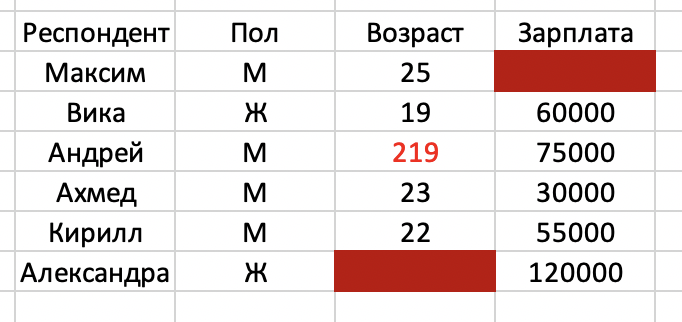
\includegraphics[scale = 0.5]{ris8.png}
	\begin{wideitemize}
		\item \textcolor{red}{Пропущенные значения} $-$ кто-то из респондентов не захотел отвечать на вопросы
		\item \textcolor{red}{Аномальные значения (выбросы)} $-$ при сборе допустилась ошибка, в следствие чего одно значение сильно отличается от остальных и не попадает в наше распределение
	\end{wideitemize}
\end{frame}

\begin{frame}{Некоторые способы решения}
	\begin{wideitemize}
		\item Построение графиков для обнаружения выбросов (плотности распределения / barplot / ... )
		\item Нахождение основных статистик для обнаружения выбросов (среднее / максимальное значение / минимальное / ... )
		\item Удаление пропущенных значений 
		\item Разумное заполнение пропущенных значений (нулями / средним / ... )
	\end{wideitemize}
\end{frame}

\begin{transitionframe}
	\begin{center}
		\Huge Трансформация данных
	\end{center}
\end{transitionframe}

\begin{frame}{Получение подтаблиц}
	Например, мы хотим вывести тех людей, которые зарабатывают меньше 80000 рублей в месяц:
	\centering 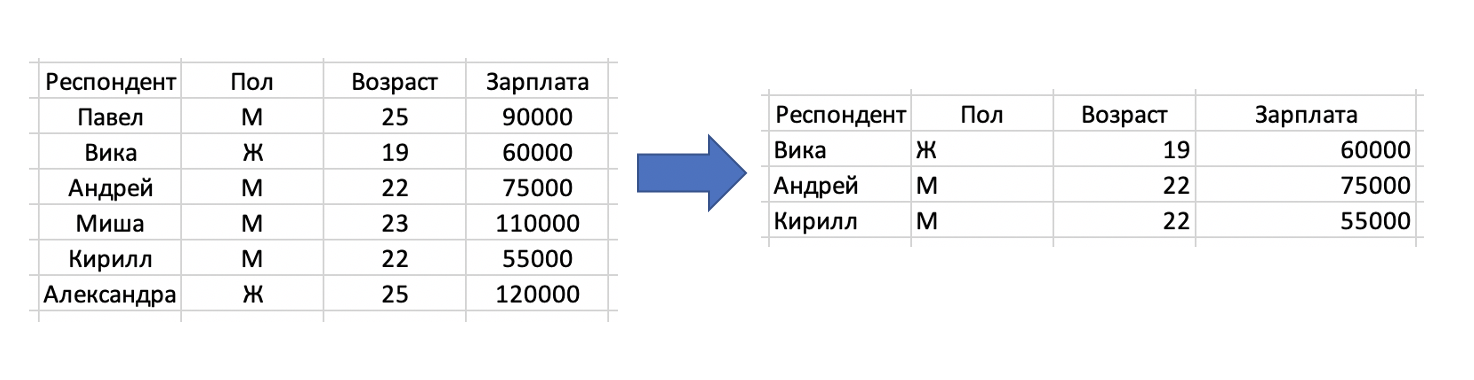
\includegraphics[scale = 0.5]{ris9.png}
\end{frame}

\begin{frame}{Агрегирование информации}
	Отдельно для мужчин и женщин хотим посчитать среднюю з/п:
	\centering 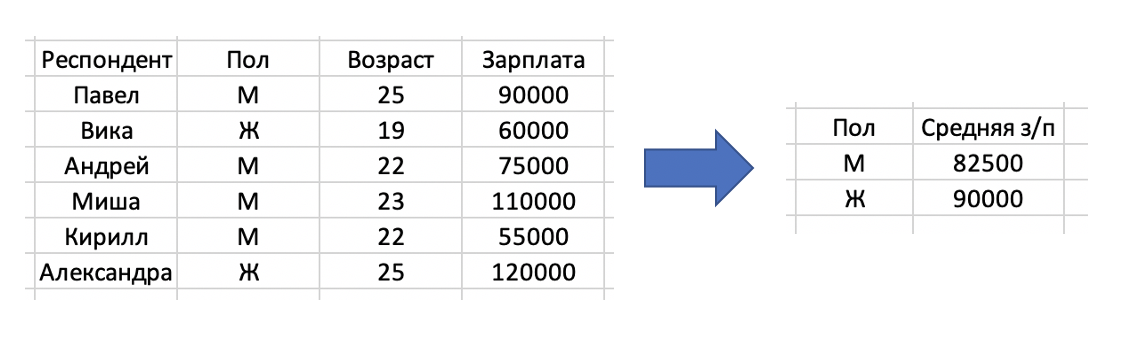
\includegraphics[scale = 0.5]{ris10.png}
\end{frame}

\begin{frame}{Объединение табличек}
	\centering 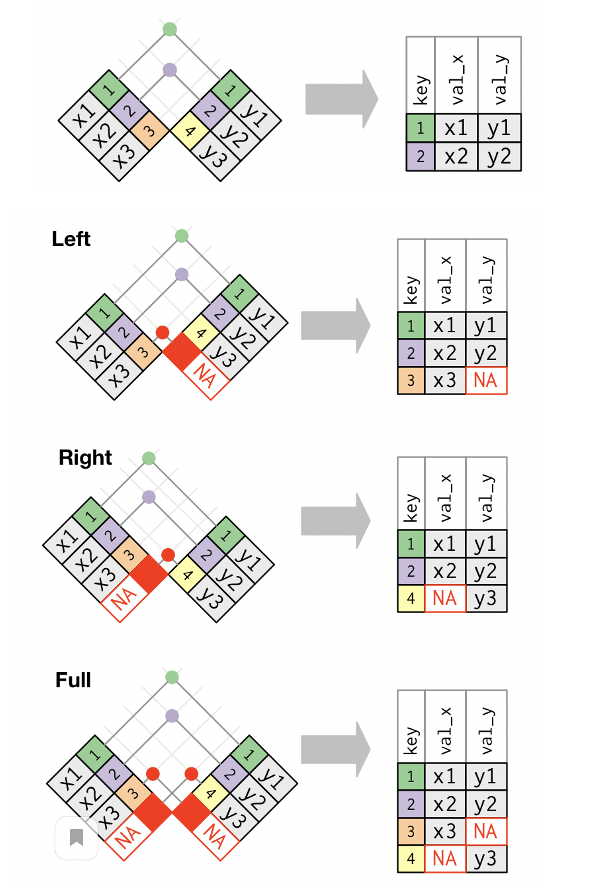
\includegraphics[scale = 0.5]{ris11.png}
\end{frame}

\begin{transitionframe}
	\begin{center}
		\Huge Модели
	\end{center}
\end{transitionframe}

\begin{frame}{Основные виды задач}
	\begin{wideitemize}
		\item \textcolor{red}{Регрессия} $-$ прогнозирование непрерывного значения (как правило это вещественное число) для конкретного наблюдения 
		\item \textcolor{red}{Классификация} $-$ отнесение наблюдения к одному из нескольких классов (частный случай: бинарная классификация)
		\item \textcolor{red}{Кластеризация} $-$ отнесение наблюдения к одному из кластеров (как правило, не знаем сколько их и как устроены)
	\end{wideitemize}
\end{frame}

\begin{frame}{Примеры задач регрессии}
	\begin{wideitemize}
		\item \textcolor{red}{Бизнес:} какая выручка магазина будет в следующем месяце? 
		\item \textcolor{red}{Экономика:} какой спрос будет на товар в следующем году? 
		\item \textcolor{red}{Анализ изображений:} сколько лет человеку на фотографии? 
		\item \textcolor{red}{Социология:} сколько человек сэмигрирует в город N? 
	\end{wideitemize}
\end{frame}

\begin{frame}{Примеры задач классификации}
	\begin{wideitemize}
		\item \textcolor{red}{Кредитный скоринг:} вернет ли клиент кредит?
		\item \textcolor{red}{Рекомендации:} понравится ли пользователю фильм? 
		\item \textcolor{red}{Медицина:} болен ли пациент? 
		\item \textcolor{red}{Биология:} к какому виду цветков относится растение?
		\item \textcolor{red}{Социология:} зарабатывают ли женщины меньше мужчин? 
		\item \textcolor{red}{Баловство:} Выживет ли пассажир на Титанике? 
	\end{wideitemize}
\end{frame}

\begin{frame}{Примеры задач кластеризации}
	\begin{wideitemize}
		\item \textcolor{red}{Тексты:} определение темы текста 
		\item \textcolor{red}{Маркетинг:} поиск схожих пользователей в социальных сетях
		\item \textcolor{red}{Социология:} выделять группы схожих анкет 
		\item \textcolor{red}{Социология:} выявлять типы людей и формировать поведенческие паттерны
	\end{wideitemize}
\end{frame}

\begin{frame}
	\begin{center}
	\textcolor{red}{Подробнее о моделях мы поговорим в следующей лекции!}
	\end{center}
\end{frame}

\end{document}